\documentclass[12pt,a4paper,titlepage]{article}
\usepackage[utf8]{inputenc}
\usepackage{polski}
\usepackage{listings}
\usepackage{graphicx}
\usepackage{xcolor}
\usepackage{minted}
\makeatletter
\newcommand{\linia}{\rule{\linewidth}{0.4mm}}
\renewcommand{\maketitle}{\begin{titlepage}
    \vspace*{1cm}
    \begin{center}\small
    Politechnika Wrocławska\\
    Wydział Elektroniki\\
    Urządzenia cyfrowe i systemy wbudowane 1
    \end{center}
    \vspace{3cm}
    \noindent\linia
    \begin{center}
      \LARGE \textsc{\@title}
         \end{center}
     \linia
    \vspace{0.5cm}
    \begin{flushright}
    \begin{minipage}{7cm}
    \textit{\small Autor:}\\
    \normalsize \textsc{\@author} \par
    \end{minipage}
    \vspace{5cm}

     {\small Wtorek, 7\textsuperscript{30}-10\textsuperscript{15} TP}\\
        Dr inż. Dariusz Caban
     \end{flushright}
    \vspace*{\stretch{6}}
    \begin{center}
   22 stycznia 2019
   % \@date
    \end{center}
  \end{titlepage}%
}
\makeatother
\author{Justyna Skalska, 225942\\
        Piotr Pawelski, 218370}
\title{Sprawozdanie nr 4\\
\large(Zamek szyfrowy w VHDL)}

\begin{document}
\maketitle

\section{Wstęp}
Celem laboratorium było zaprojektowanie automatu otwierającego zamek szyfrowy w języku VHDL. Hasło składało się z 2 cyfr: 122. Przyciski znajdujące się na płytce odpowiadały poszczególnym cyfrom od 1 do 8. Zaświecenie się wszystkich diód oznaczało poprawne otwarcie zamka szyfrowego.\\\\
Programem wykorzystanym do wykonania zadania jest ISE Design Suite.

\section{Przebieg zajęć}
Zajęcia rozpoczęliśmy zaprojektowania stanów automatu oraz przejść pomiędzy nimi. Następnie zaprogramowaliśmy je w języku VHDL wraz z odpowiednimi wejściami i wyjściami. 



\begin{listing}[H]
\caption{Kod VHDL}
\begin{minted}[linenos,breaklines]{vhdl}

library IEEE;
use IEEE.STD_LOGIC_1164.ALL;


entity FST is
    Port ( Key : in  STD_LOGIC_VECTOR (0 to 7);
           Clk : in  STD_LOGIC;
           Output : out  STD_LOGIC_VECTOR (0 to 7));
end FST;

architecture Behavioral of FST is

   type state_type is ( A, A1, B, B1, C, C1, D );
   signal state, next_state : state_type;
begin
   
   process1 : process( Clk )
   begin
      if rising_edge( Clk ) then
      
         state <= next_state;
      
      end if;
      
   end process process1;

   process2 : process( state, Key )
   begin
      next_state <= state; -- by default
      
      case state is
      
      when A =>
         if Key = "00000001" then
            next_state <= A1;
         end if;
  \end{minted}
\end{listing}
\newpage
\begin{listing}[H]
\caption{Kod VHDL}
\begin{minted}[linenos,breaklines]{vhdl}       
      when A1 =>
         if Key = "00000000" then
            next_state <= B;
         end if; 
      
      when B =>
         if Key = "00000010" then
            next_state <= B1;
         elsif Key = "00000000" then
            next_state <= B;
         else
            next_state <= A;
         end if;

      when B1 =>
         if Key = "00000000" then
            next_state <= C;
         end if; 
         
      when C =>
         if Key = "00000010" then
            next_state <= C1;
         elsif Key = "00000000" then
            next_state <= C;
         else
            next_state <= A;
         end if;
         
      when C1 =>
         if Key = "00000000" then
            next_state <= D;
         end if;
           \end{minted}
\end{listing}
\newpage
\begin{listing}[H]
\caption{Kod VHDL}
\begin{minted}[linenos,breaklines]{vhdl}       
      when D =>
         if Key = "00000001" then
            next_state <= A1;
         elsif Key = "00000000" then
            next_state <= D;
         else
            next_state <= A;
         end if;

      end case;

   end process process2;

   process3 : process( state )
   begin
      
      
      case state is
      
      when A =>
         Output <= "11111110"; 
         
      when A1 =>
         Output <= "11111101"; 
      
      when B =>
         Output <= "11111011";
         
      when B1 =>
         Output <= "11110111";
         
      when C =>
         Output <= "11101111";
          \end{minted}
\end{listing}
\newpage
\begin{listing}[H]
\caption{Kod VHDL}
\begin{minted}[linenos,breaklines]{vhdl}        
      when C1 =>
         Output <= "11011111";
         
      when D =>
         Output <= "00000000";

      end case;

   end process process3;


end Behavioral;


\end{minted}
\end{listing}

Kolejnym etapem było wygenerowanie symbolu naszej maszyny stanów oraz stworzenie prostego schematu na którym dołączyliśmy do niej wejścia i wyjścia.

\begin{figure}[H]
\centering
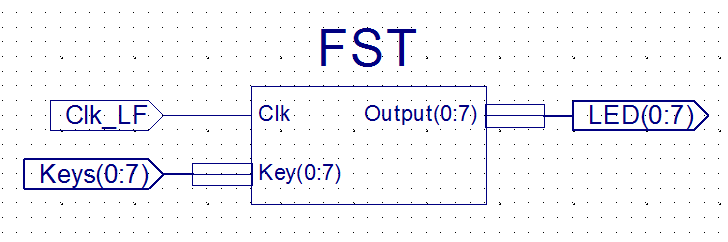
\includegraphics[angle=90,height=20cm]{fst.png}
\caption{Schemat układu}
\label{fig:schemat}
\end{figure}



\begin{itemize}
    \item \textbf{Keys(0:7)} to kolejne przyciski odpowiadające cyfrom od 1 do 8
    \item \textbf{Clk\_LF} to wejście układu odpowiadające za dostarczenie sygnału zegara.
    \item \textbf{LED(0:7)} to diody, które pokazują w jakim stanie znajduje się obecnie układ oraz czy zamek został otwarty
\end{itemize}
Następnym zadaniem, które wykonaliśmy było skompilowanie układu oraz wygenerowanie pliku .jed, który jest używany do programowania mikroprocesorów. Następnie przesłaliśmy nasz program na płytkę, gdzie udało nam się poprawnie wpisać szyfr oraz otworzyć zamek.

\section{Wnioski}
Podczas laboratoriów mogliśmy zapoznać się z podstawami tworzenia automatów w języku VHDL przy użyciu programu ISE Design Suite.
\end{document}